\section{Pure Approach}
The section summarise the results of the pure crowdsourcing experiments. First, the overall performance of the pipeline is evaluated. After that, the results of the four subtask are assessed.
\subsection{Overall Performance}
After all the necessary content was created by the crowd, the evaluation was done by comparing the ground truth with the generated information. The evaluation task presented the fields title, description and category to the workers. They had to decide which auction description is the best one in their opinion. The result is illustrated in figure \ref{crowdsourcing_eval}. The commission approach got a majority of the votes with 57.14\%. The generic item received all five votes from the crowd. The ground truth contains unnecessary information and looks like a scam, is the statement of the participants.

The workers had the possibility to reason their decision. They motivate their votes as follows: 
\begin{itemize}
	\item Higher value of information 
	\item Professionalism 
	\item Hidden information are given (e.g. size of the cleats, size of the smartphone storage) 
	\item The description is clear, short and to the point 
	\item Authenticity of the article 
	\item Grammatical issues 
\end{itemize}
\begin{figure}
\centering
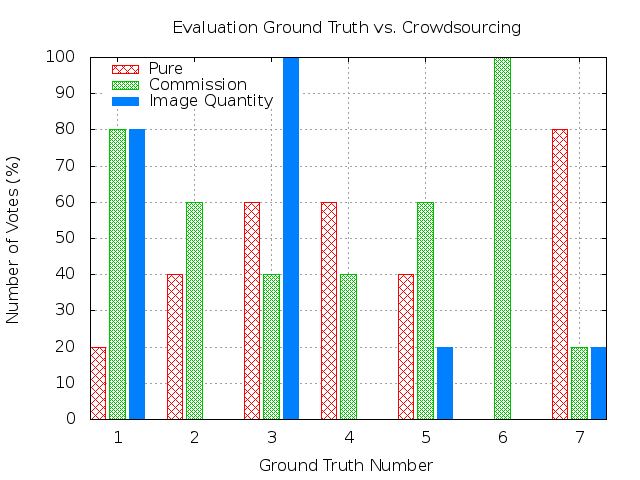
\includegraphics[scale=0.55]{images/plots/crowdsourcing/plot_evaluation_all.png}
\caption{Evaluation of ground truth vs. crowdsourcing}
\label{crowdsourcing_eval}
\end{figure}
\subsection{Title}
The length of the title (Figure \ref{crowdsourcing_title_length}) increases if the task contains all available pictures of the item. This setup produced an average title length of 64 characters. The other experiments have an average of 50 for the standard design and 48 for a promised commission. The median value shows almost the same ranking except the additional reward in form of a commission generates more characters than the standard configuration. The item without a brand was described by a title with 37 characters. The length doesn't say anything about the quality of the title, but it indicates the influence of the different task settings. The usage of natural language processing tools could help to get more information about the quality, but this would be outside the scope of the thesis.
\begin{figure}
\centering
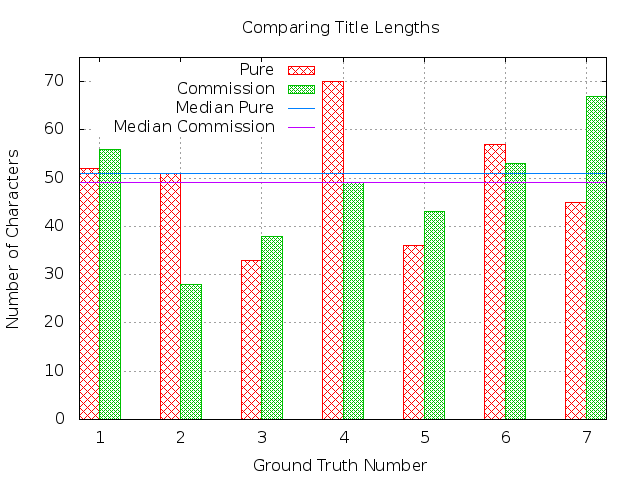
\includegraphics[scale=0.55]{images/plots/crowdsourcing/plot_title_length.png}
\caption{Evaluation of title lengths}
\label{crowdsourcing_title_length}
\end{figure}
The workers spent more time to find a title if they can achieve an additional bonus (Figure \ref{crowdsourcing_time_title}). The average working time (203.76 seconds) is twice as much as without a commission (101.76 seconds). If the writer of the title has to look at more than the three standard images then they needed more time to commit a title (131.28 seconds). If the additional time effort was used to open all the supplementary images is not clear at the moment.

After the creation of the titles, the workers had to select the final one for each item. They justify their selections as follows:
\begin{itemize}
	\item Amount of details 
	\item Attracts more attention 
	\item Research on eBay produces better results for the title 
	\item Experiences with online auctions 
	\item Wrong information 
	\item Too long 
\end{itemize}
\begin{figure}
\centering
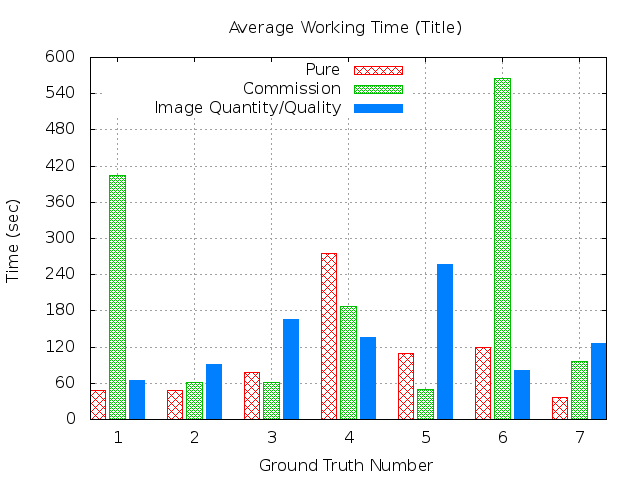
\includegraphics[scale=0.55]{images/plots/crowdsourcing/plot_time_title.png}
\caption{Evaluation of the average working times for finding a title}
\label{crowdsourcing_time_title}
\end{figure}
\subsection{Description}
The same measurements as for the title were done for the description (Figure \ref{crowdsourcing_desc_length}). The general task design achieved the highest average length (467 chars), but it contains an outlier with 1'706 characters for the ground truth item number 5. The worker copied an item description from the website of the producer. More images doesn't conclude to a longer description, because the average length of these titles is 281. An extra reward leads to 455 characters, but has the highest median of 572. The numeric parameter is more robust to outliers. The other setups follow by 307 (Commission) and 238 (Pure). The non-branded item realise a length of 240 characters which is equal to the median of the branded items. Therefore, the workers are able to write descriptions of equal length regardless of which item type (branded/non-branded) was presented to them.
\begin{figure}
\centering
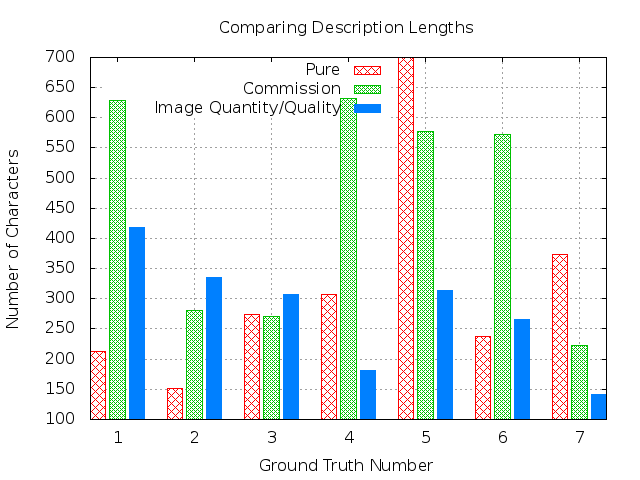
\includegraphics[scale=0.55]{images/plots/crowdsourcing/plot_description_length.png}
\caption{Evaluation of description lengths}
\label{crowdsourcing_desc_length}
\end{figure}

\subsection{Category}
Most of the workers submitted only the main category and not the complete hierarchy with main and sub categories. For the football trading cards they wrote ``Sports Mem, Cards \& Fan Shop'' instead of ``Sports Mem, Cards \& Fan Shop:Cards:Football'', for example. One reason could be that the instructions weren't clear and precise enough. Also the desired format of the input wasn't mentioned. An improved task design will result in more accurate outputs.
\subsection{Price Estimation}
To evaluate the accuracy of the price estimations (Figure \ref{crowdsourcing_price_pred}), the root mean squared error (RMSE) was used. It is frequently used to measure the quality of predictions. The true values are the end prices from the ground truth. If the workers have the actual market price of the item at one's disposal then they predict the price best with an average RMSE of 51.46 USD. The experiment with the commission ranked just behind with 58.55 USD, the others appear with 81.75 (Pure) and 89.89 (Image quantity/quality) at the end of the ranking. The tested item without a brand has a RMSE of 1074.12 USD. The comparison between branded and non-branded items can be done by dint of the absolute percentage error. The value represents the difference between predicted and exact value as a percentage of the exact value. The seven ground truth items have an error of 51\% in median, the non-branded item one of 83\%. The values from the branded items are taken from the standard experiment to have the same preconditions for both categories. The results indicate the challenge of the price prediction for generic things.

The digital watch and the handbag have a lot of predictions which are higher than the ground truth price (Figure \ref{crowdsourcing_price_overestimations}). Reasons could be that the watch was sold at a cheaper price than expected and the handbag could be a fake.

The estimation errors can be explained by different observations. The size of the smartphone storage isn't given. The price difference of an iPhone 5S with 32GB and 64GB is about 100 dollars. The football trading cards are difficult to estimate, because most of the workers don't know the football players and cannot asses the rarity or popularity of them. The football boot model is available in different versions. The original one and cheaper replicas. The action figure is rare and no other auctions are available to compare with.

The results of the expenditure of time for the price estimations (Figure \ref{crowdsourcing_time_price}) are disappointing. The workers spent between 155 (Pure) to 493 (Image quantity/quality) seconds on average to find an appropriate price for the items. The promised commission had only a marginal influence on the time statistic.
\begin{figure}
\centering
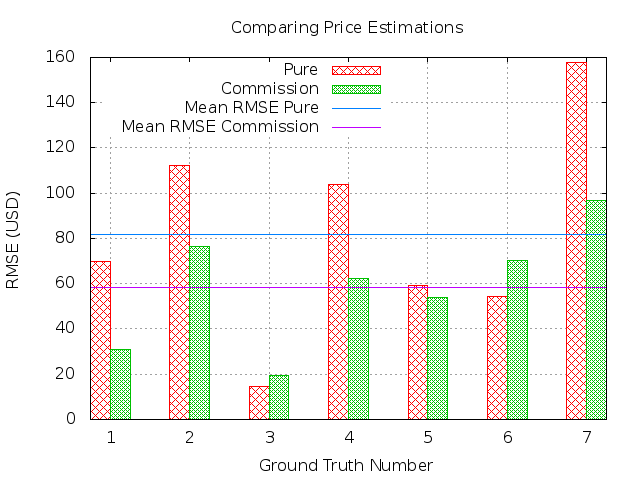
\includegraphics[scale=0.55]{images/plots/crowdsourcing/plot_price_rmse.png}
\caption{Price prediction quality}
\label{crowdsourcing_price_pred}
\end{figure}
\begin{figure}
\centering
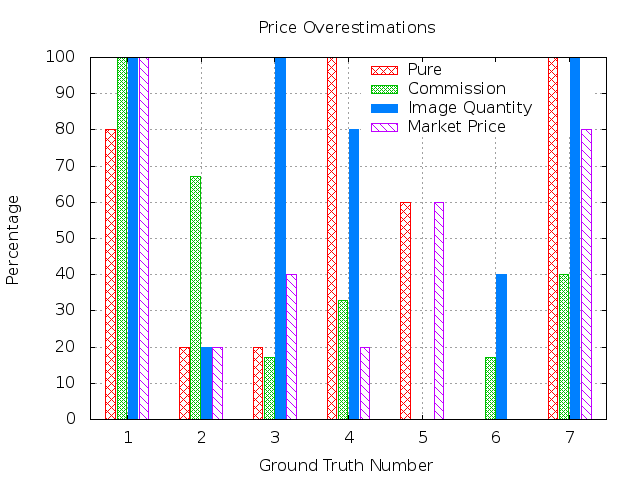
\includegraphics[scale=0.55]{images/plots/crowdsourcing/plot_price_overestimation.png}
\caption{Price overestimations}
\label{crowdsourcing_price_overestimations}
\end{figure}
\begin{figure}
\centering
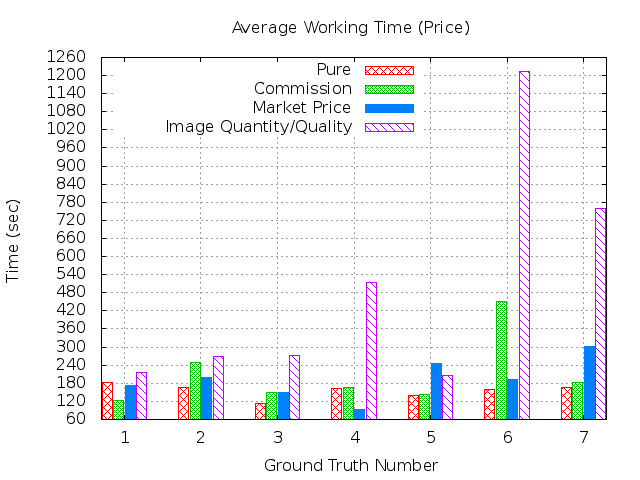
\includegraphics[scale=0.55]{images/plots/crowdsourcing/plot_time_price.png}
\caption{Evaluation of the average working times for the price estimation}
\label{crowdsourcing_time_price}
\end{figure}
\subsection{Variations}
\subsubsection{Commission}
The ground truth items 1 and 3 received a majority of the votes from the crowd. The commissions were paid manually using the web interface of the Amazon Mechanical Turk web service. The value of the bonus has to be shortened to two digits after the point and rounded up to \$0.01, because of some restrictions of MTurk. The bonus aggregates to \$1.48 for both auctions (see table \ref{tab_commission}, page \pageref{tab_commission}). The workers also received an additional message:\\\\
``Dear worker, \\\\
You receive a commission (0.25\% of the end price) as bonus payment for your work. The end price of the eBay online auction was \$27.''
\section{Hybrid Approach}
The Random Forest approach shows the best performance over all three item categories independent of classification or regression (Figure \ref{class_acc}/\ref{reg_rmse}). The results of three iterations were averaged, because of the randomness of the classifier. The accuracy of the classifier depends also on the item category. The RFC assigns every third input to the right Sony Playstation price class. The plot of the mean absolute error (MAE, Figure \ref{class_mae}) assures the strength of the classifier and visualises how far away the predictions are in average. kNN has an error of about four classes for the iPhone category, one class has a range of 25 USD.

The reasons for the moderate performance of the classifiers could be multi-object and/or outdated auctions in the collected data. A higher number of features could also lead to better results.

The comparison between the human-based and the machine-based prediction isn't possible with the aid of the RMSE, because the values are scale-dependent. But, the random forest algorithm predicts a final price of the ground truth item number 2 (Apple iPhone) of \$108 and the crowd a price of \$172. The crowdsourced price is taken from the experiment where the workers had access to the market price, because this experiment has the lowest error rate. The ground truth price is \$185. The crowd has an absolute price difference of \$13, the machine learning approach one of \$77. The mean absolute error confirms this observation. Five workers predicted prices with an error of 21\%, the machine learning approach one of 30.9\%.

The normalised confusion matrix (Figure \ref{conf_mat_iphone}) of the iPhone classifiers illustrates the distribution of the assignments. The origin is located at the left top position, the x-axis represents the truth-values and the y-axis the values assigned by the classifier. The values were normalised per row. A perfect classifier would produce a diagonal which contains only ones. 
The scatter plot (Figure \ref{true_predict_iphone}) is another way to visualise the relations between the truth and predicted values. The criteria of a perfect classifier are the same as for the confusion matrix. 
The same plots for the other categories and the exact accuracies/RMSEs/MAEs are enumerated in the appendix section.
\begin{figure}
\centering
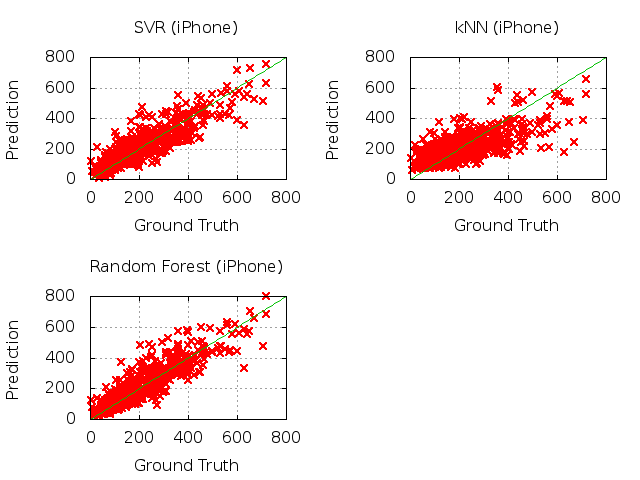
\includegraphics[scale=0.55]{images/plots/machine_learning/iphone/true_pred_iphone.png}
\caption{Scatter plot true vs. prediction (iPhone)}
\label{true_predict_iphone}
\end{figure}
\begin{figure}
\centering
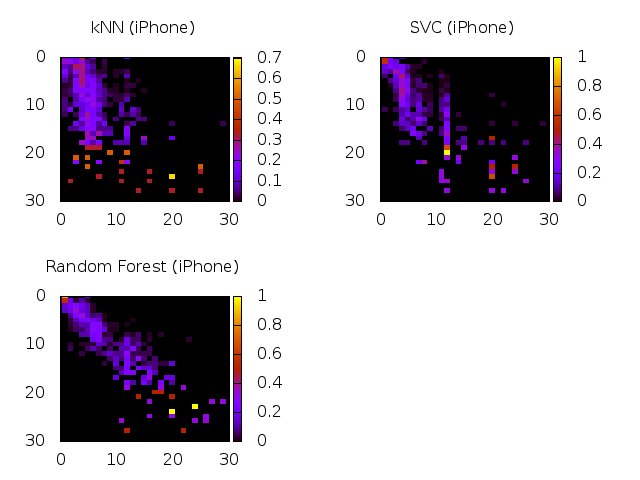
\includegraphics[scale=0.55]{images/plots/machine_learning/iphone/conf_mat_iphone.png}
\caption{Normalised confusion matrix (iPhone)}
\label{conf_mat_iphone}
\end{figure}

\begin{figure}
\centering
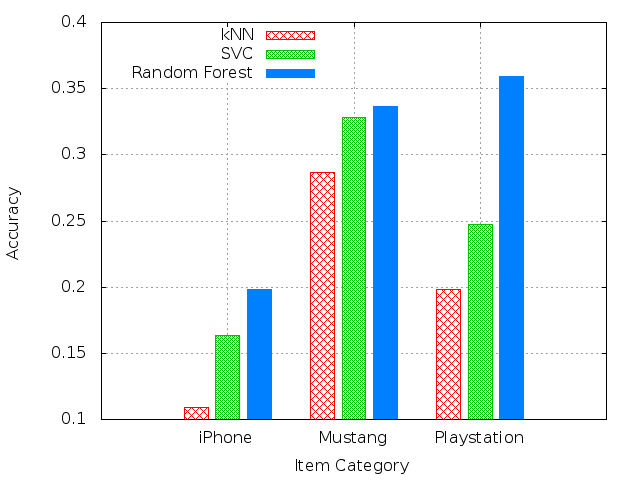
\includegraphics[scale=0.55]{images/plots/machine_learning/plot_price_classification_acc.png}
\caption{Classification accuracy}
\label{class_acc}
\end{figure}
\begin{figure}
\centering
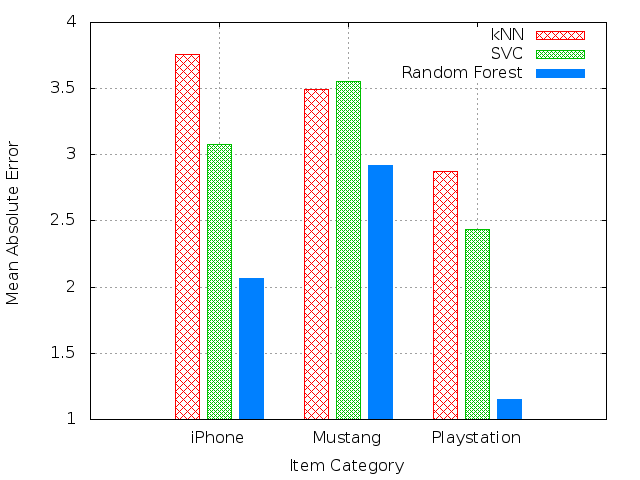
\includegraphics[scale=0.55]{images/plots/machine_learning/plot_price_classification_mae.png}
\caption{Classification mean absolute error}
\label{class_mae}
\end{figure}

\begin{figure}
\centering
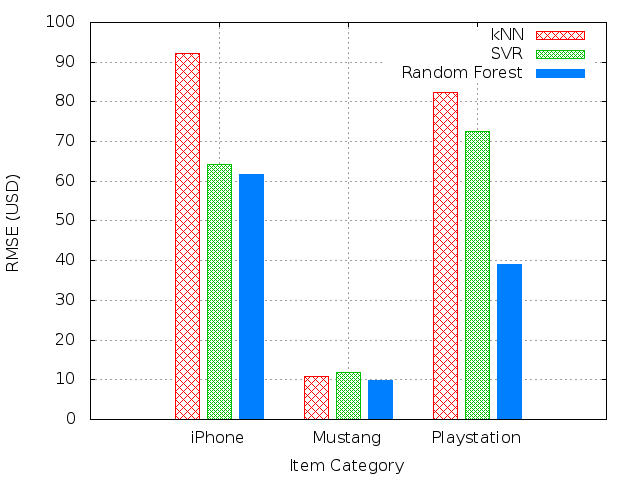
\includegraphics[scale=0.55]{images/plots/machine_learning/plot_price_regression_rmse.png}
\caption{Regression root mean squared error}
\label{reg_rmse}
\end{figure}



